%!TEX program = xelatex
\documentclass{beamer}
%\documentclass[aspectratio=169]{beamer} %如果需要16:9
\usepackage{ctex}
\usepackage{times}
\usepackage{multicol}
\usepackage{multirow}
\usetheme{Warsaw}
\usepackage{tikz}
\usetikzlibrary{arrows,shapes,chains}
\usepackage[super,square]{natbib}
%\usecolortheme{beaver}     % use white-grey colour style
%\beamersetaveragebackground{black!10}
% This is only inserted into the PDF information catalog. Can be left out.
\subject{presentation}
\keywords{example}
\useinnertheme{circles}%{rectangles}
\setbeamertemplate{itemize item}{$\circledast$}%{\checkmark}

%% ======================================================
%%     preamble
%% ======================================================
\title{基于SpringMVC架构WEB应用系统优化研究}
\author{武斌}
\institute
{
  电子系~中国海洋大学
  \and
   Department electronic engineering \\
  Ocean University Of China
}
% \date{\today}
\date{2017年5月25日}

\logo{
\includegraphics[height=0.09\textwidth]{./logo/Ocean_University_of_China.png}}


%% ======================================================
\begin{document}

%% ++++++++++++++++++++++++++++++++++++++++++++++++++++++
%% title page
%% ++++++++++++++++++++++++++++++++++++++++++++++++++++++
\begin{frame}
  \titlepage
\end{frame}

%% ++++++++++++++++++++++++++++++++++++++++++++++++++++++
%%     Table of Contents
%% ++++++++++++++++++++++++++++++++++++++++++++++++++++++
%\begin{frame}
    %\frametitle{Contents}
    %\tableofcontents
    %% 显示1-4section,不显示subsection
    %\tableofcontents[hidesubsections,sections={<1-4>}]
%\end{frame}

%% ++++++++++++++++++++++++++++++++++++++++++++++++++++++
%%     目录
%% ++++++++++++++++++++++++++++++++++++++++++++++++++++++
%\section{概述}
\begin{frame}
  \frametitle{目录}
  \begin{enumerate}
    \item<1-> 研究目的及意义
    \item<1-> 研究方法及内容
    \item<1-> 研究结论及评价
    \item<1-> 后续工作安排
  \end{enumerate}
\end{frame}


%% ++++++++++++++++++++++++++++++++++++++++++++++++++++++
%%      正文
%% ++++++++++++++++++++++++++++++++++++++++++++++++++++++
%% ++++++++++++++++++++++++++++++++++++++++++++++++++++++
%%      选题背景
%% ++++++++++++++++++++++++++++++++++++++++++++++++++++++
%\section{选题来源和背景分析 }
%\subsection{系统结构}
\begin{frame}
  \frametitle{目的及意义}
  \begin{block}{研究目的}
  	\begin{itemize}
  		\item 研究一种切实可用的WEB平台运维优化方案
  		\item 海信实习过程中参与小微系统开发、环境部署与优化的工作
  	\end{itemize}
  \end{block}
  \begin{block}{研究意义}
  	\begin{itemize}
  		\item 基于WEB技术开发一款服务于大学生创新创业的网络平台
  		\item 研究系统开发过程中的代码、持续集成、负载等方面的优化策略
  	\end{itemize}
  \end{block}
\end{frame}

%% ++++++++++++++++++++++++++++++++++++++++++++++++++++++
%%      研究内容
%% ++++++++++++++++++++++++++++++++++++++++++++++++++++++
\begin{frame}
  \frametitle{方法及内容}
  \begin{enumerate}
    \item<1-> 研究的基本框架
    \item<1-> 应用性能优化
    \item<1-> 数据库性能优化
    \item<1-> 服务器稳定性优化
  \end{enumerate}
\end{frame}

\begin{frame}
  \frametitle{平台开发基本框架}
  \begin{figure}
  \centering
    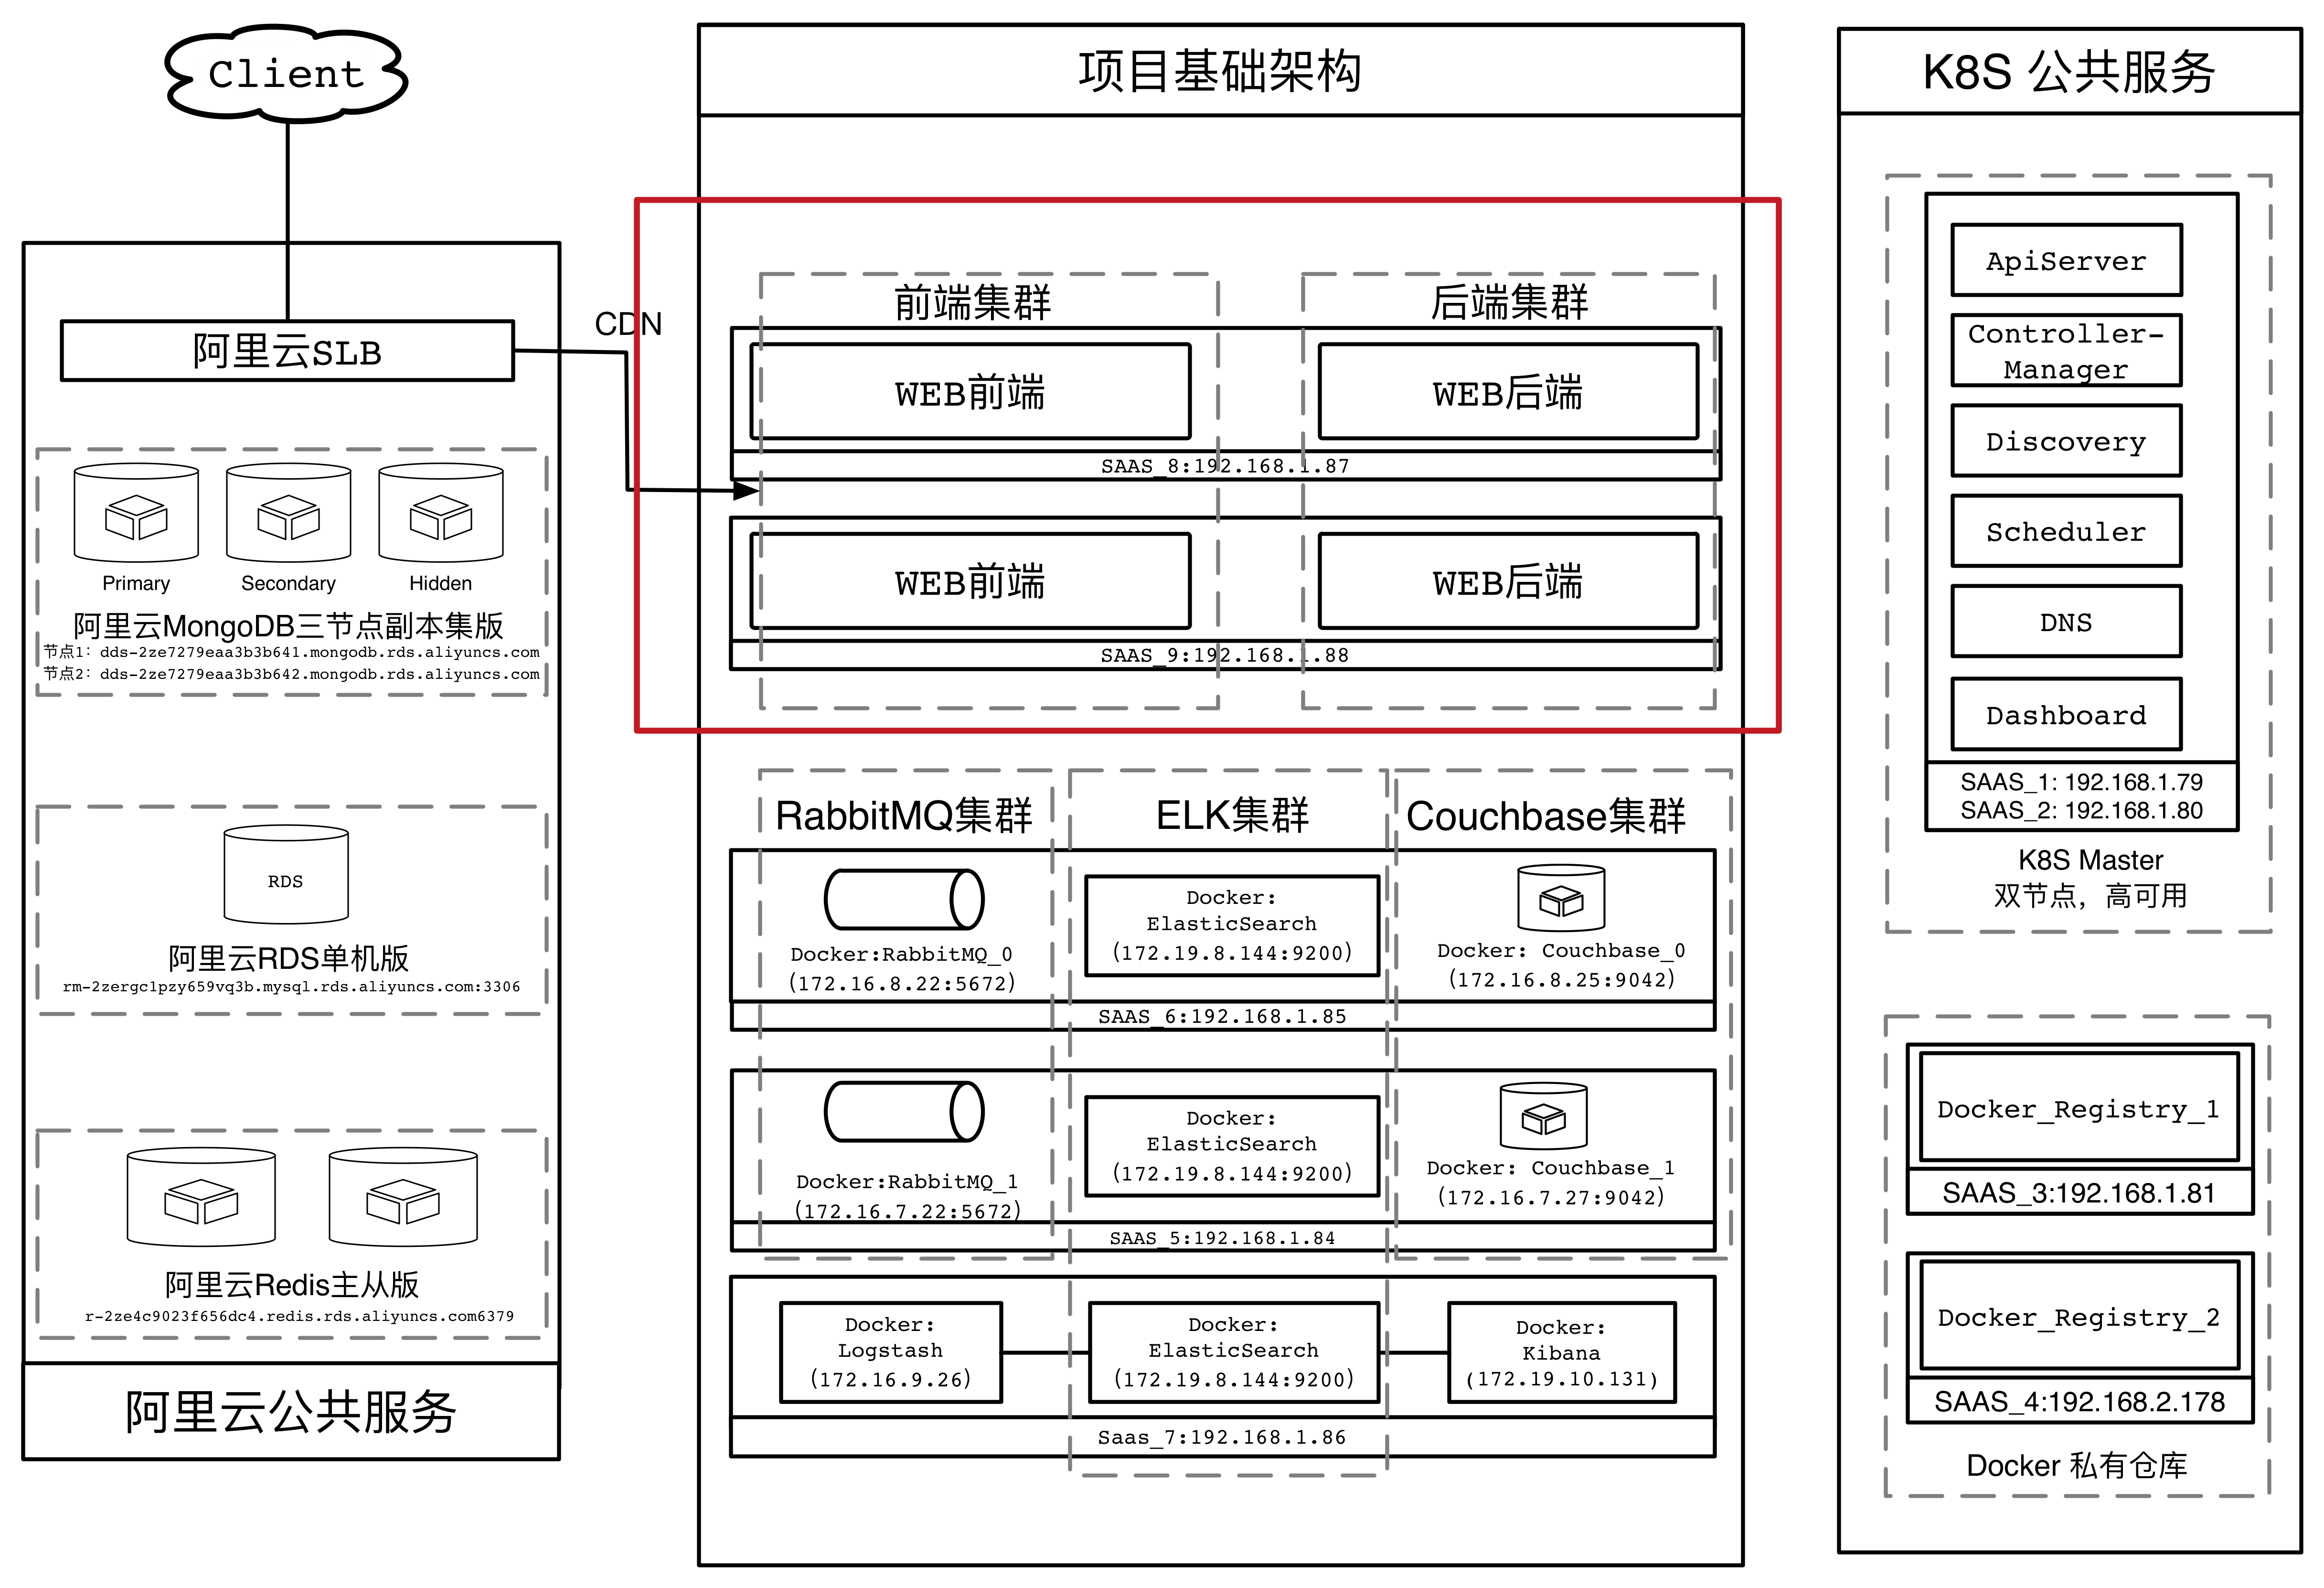
\includegraphics[height=6cm]{./img/02/deploy.png}
    \caption{平台开发基本框架}
    \label{fig:deploy}
  \end{figure}
\end{frame}

\begin{frame}
  \frametitle{研究的主要内容}
  \begin{figure}
  \centering
    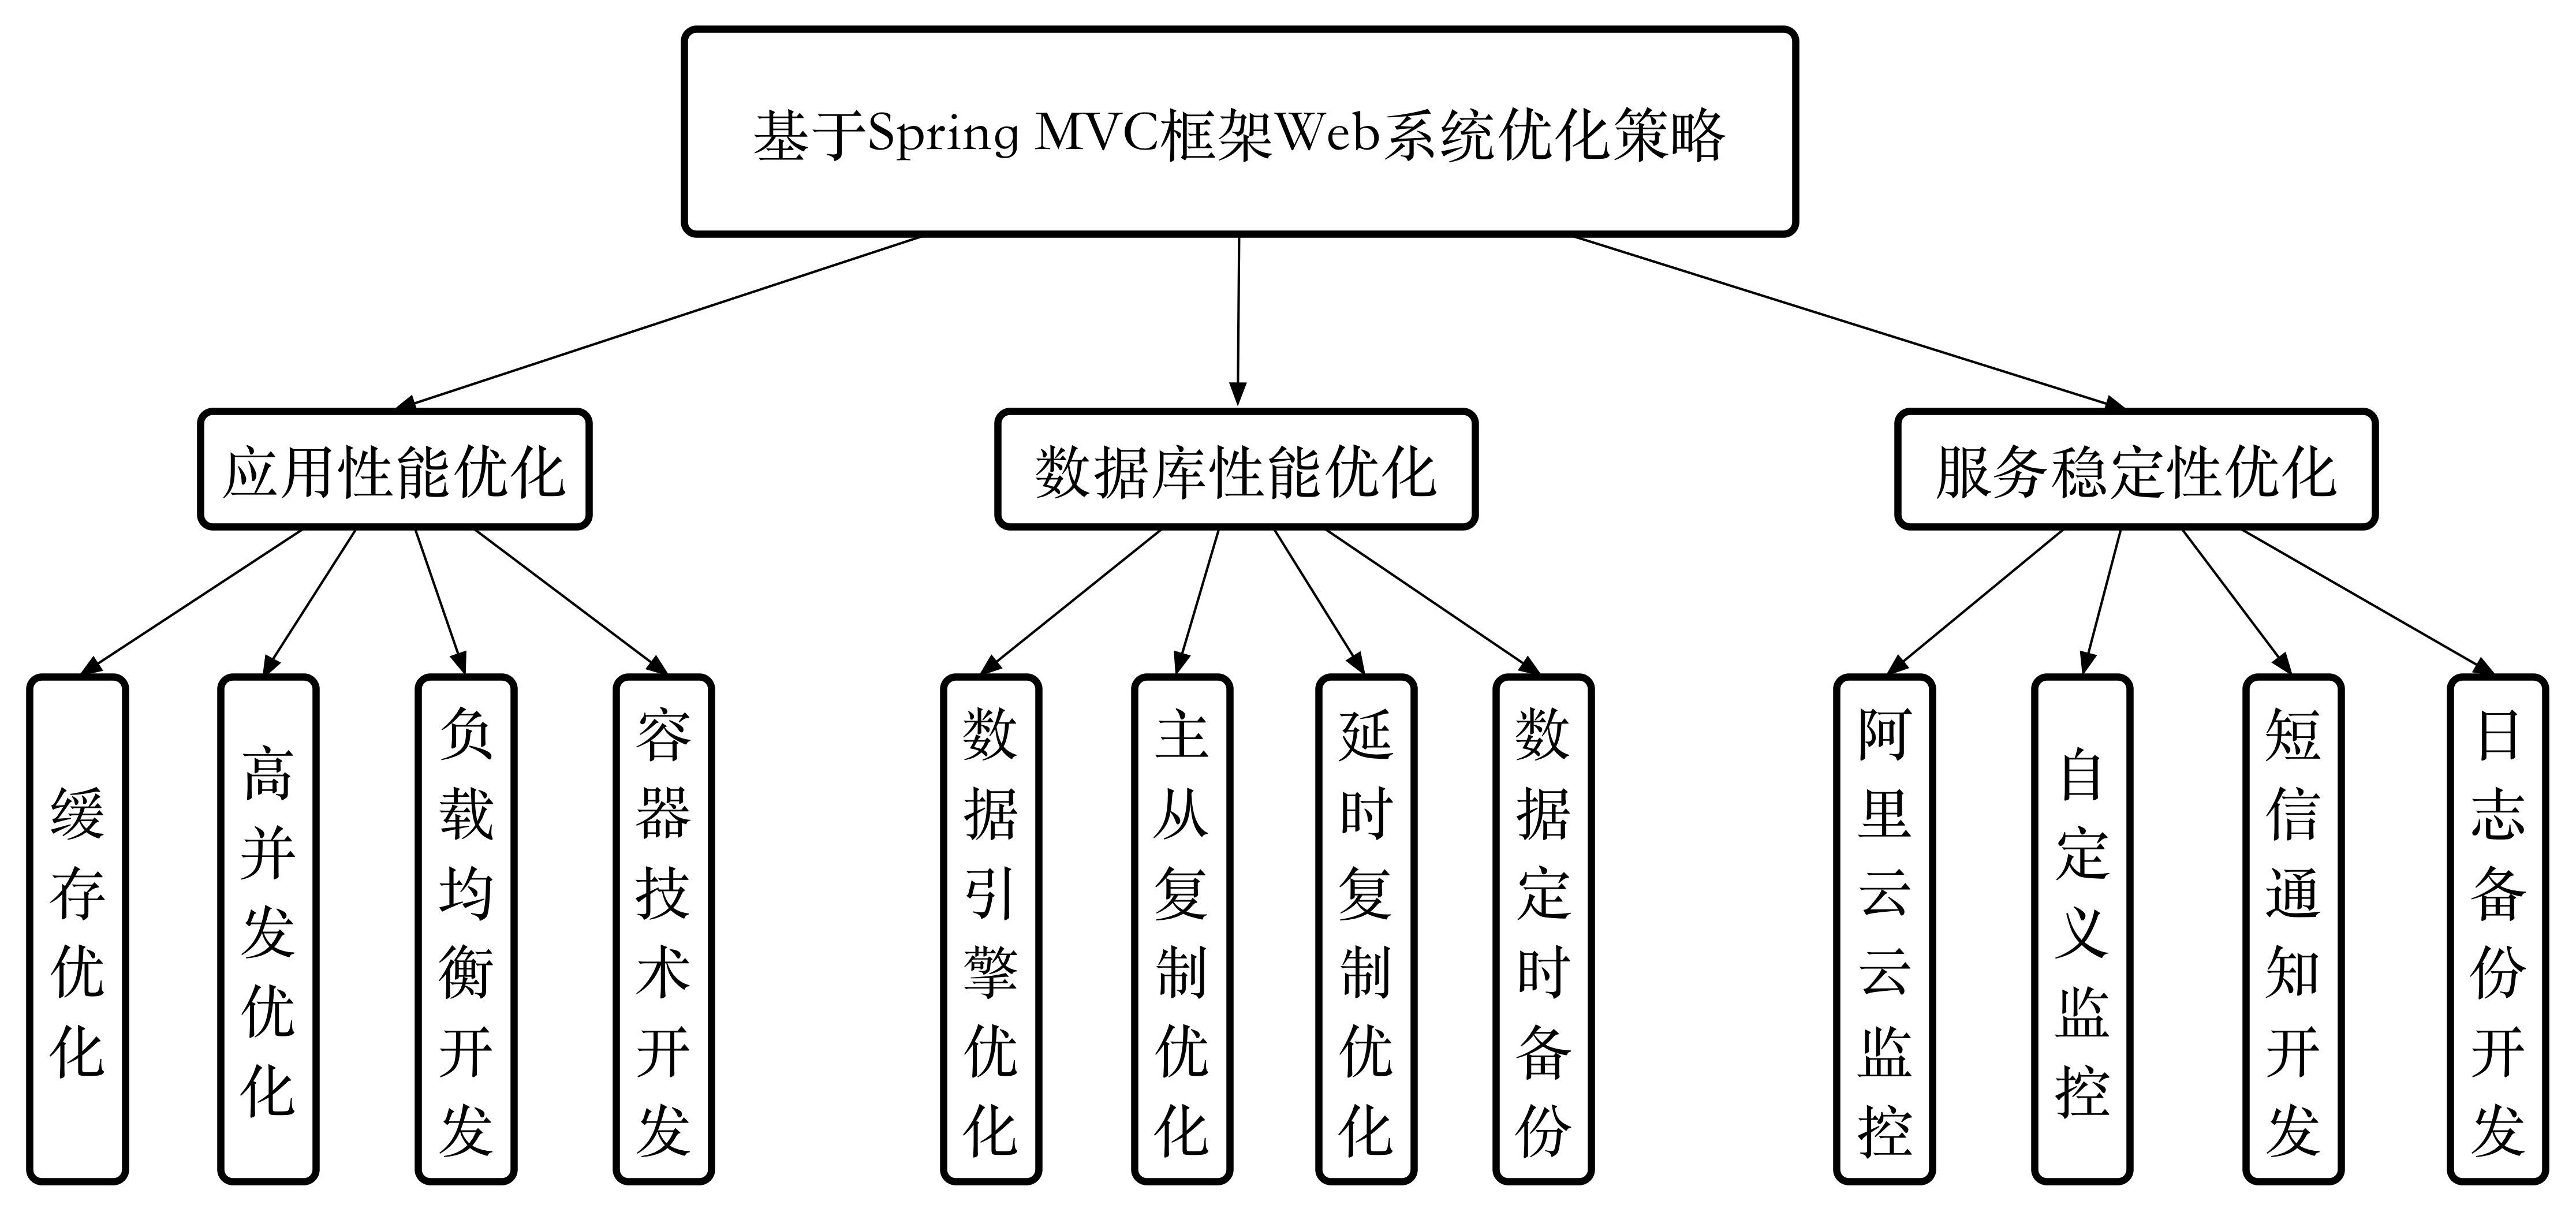
\includegraphics[height=5cm]{./img/02/summery.png}
    \caption{平台功能}
    \label{fig:summery}
  \end{figure}
\end{frame}

\begin{frame}
  \frametitle{应用性能优化}
  \begin{columns}
    \begin{column}{0.50\textwidth}
      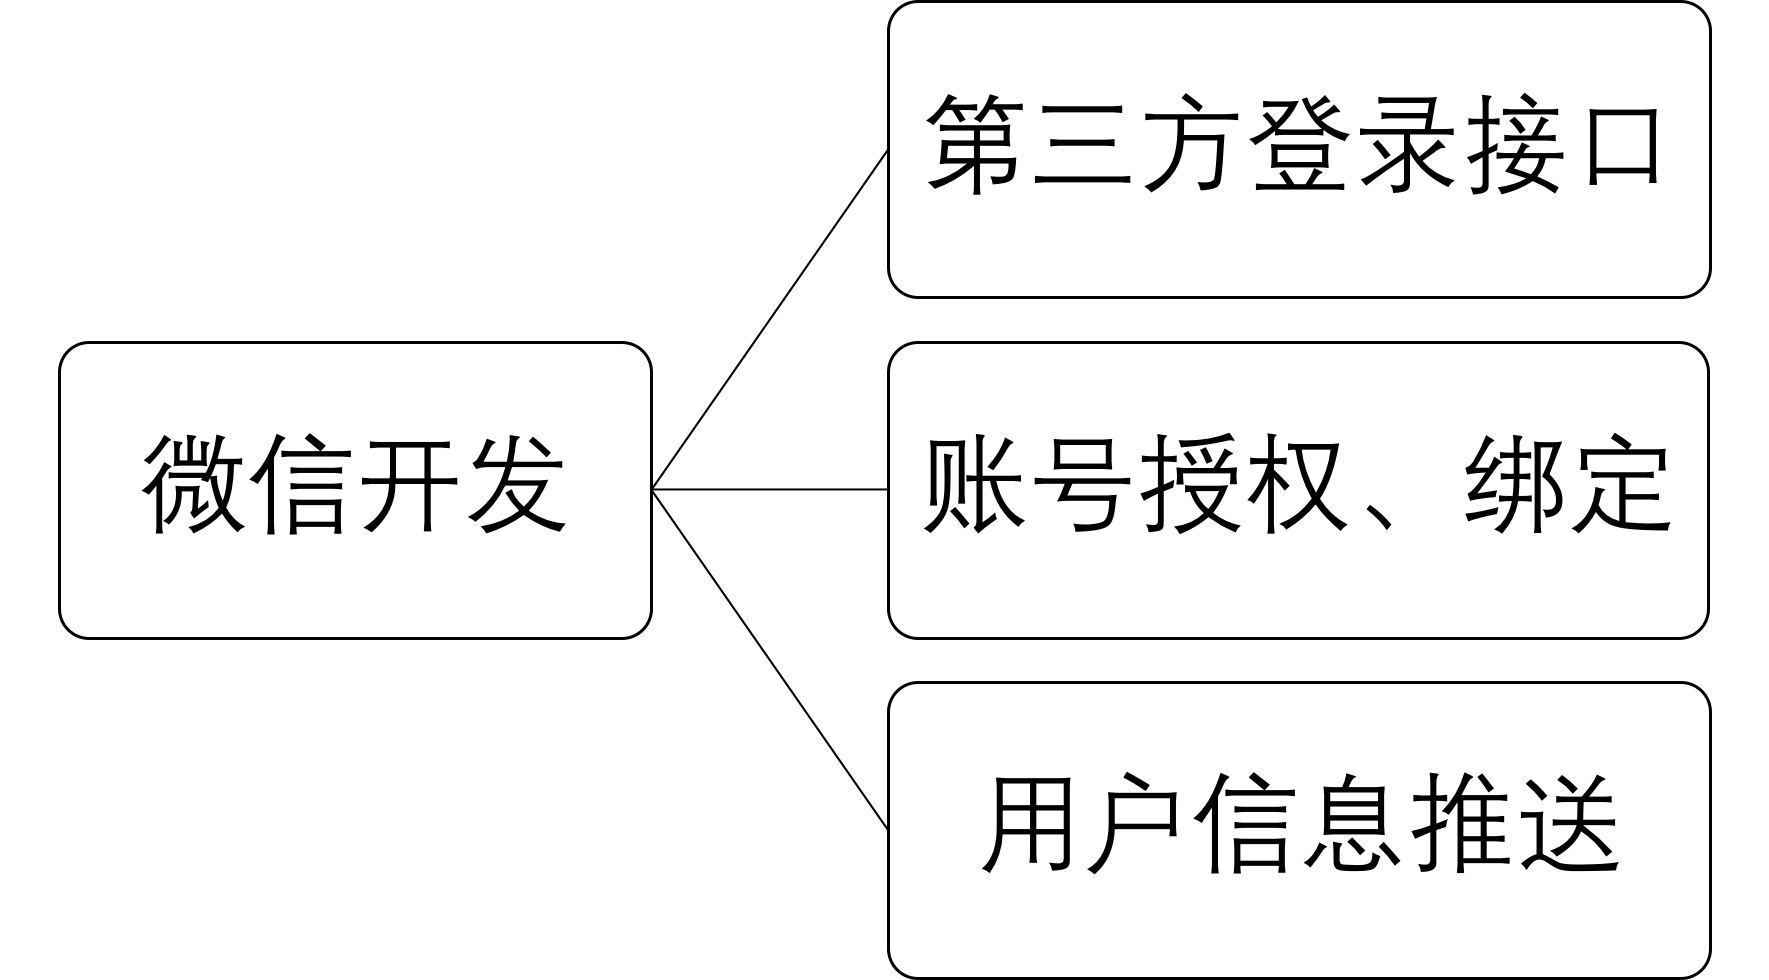
\includegraphics[width=\textwidth]{./img/web_weixin.png}
    \end{column}
    \begin{column}{0.50\textwidth}
      \begin{block}{开发目标}
        \begin{enumerate}
          \item 针对不同用户完成不同功能模块的开发
          \item 实现微信端的浏览、访问、授权
          \item 实现针对定向用户的个性化推荐
        \end{enumerate}
      \end{block}
    \end{column}
  \end{columns}
\end{frame}

\begin{frame}
  \frametitle{应用性能优化}
  \begin{columns}
    \begin{column}{0.50\textwidth}
      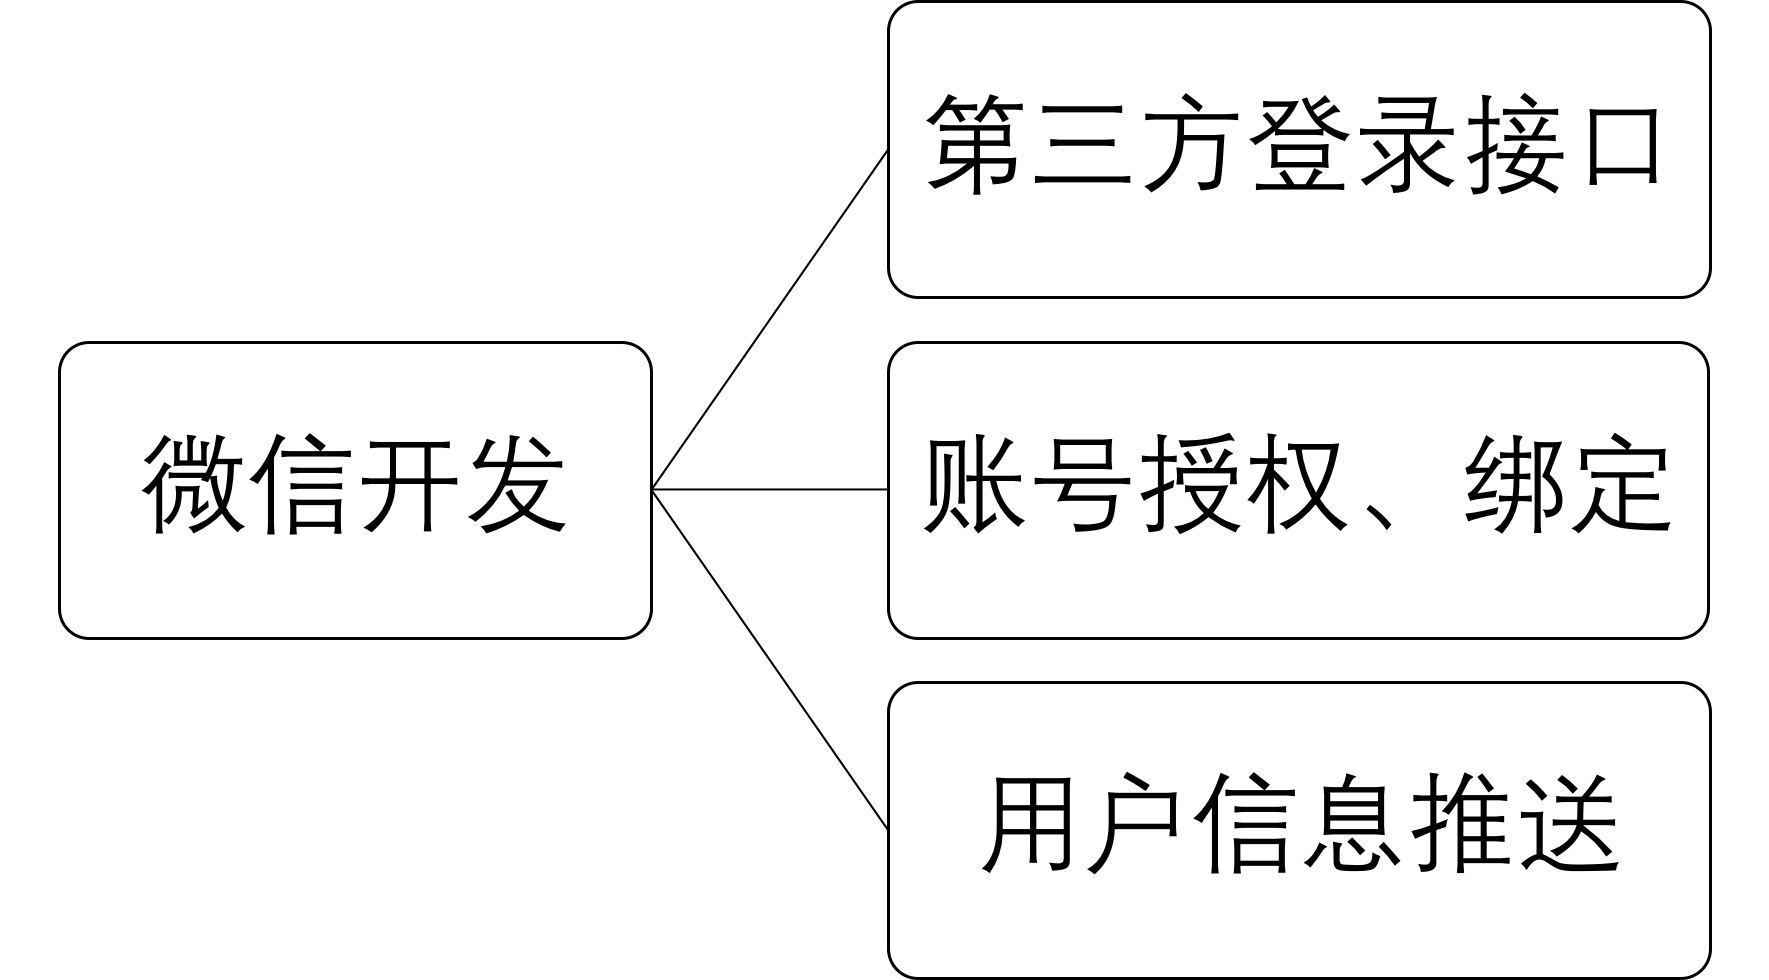
\includegraphics[width=\textwidth]{./img/web_weixin.png}
    \end{column}
    \begin{column}{0.50\textwidth}
      \begin{block}{开发目标}
        \begin{enumerate}
          \item 针对不同用户完成不同功能模块的开发
          \item 实现微信端的浏览、访问、授权
          \item 实现针对定向用户的个性化推荐
        \end{enumerate}
      \end{block}
    \end{column}
  \end{columns}
\end{frame}

\begin{frame}
\frametitle{数据库性能优化}
  \begin{block}{推荐系统开发}
  	\begin{itemize}
  		\item 探索基于平台用户数据的推荐系统开发,实现学生用户的融资求职机会推荐和企业用户的创业项目推荐
  	\end{itemize}
  \end{block}
\end{frame}

\begin{frame}
  \frametitle{服务器稳定性优化}
  \begin{block}{持续集成环境构建 }
    \begin{itemize}
      \item 通过境搭建一个持续集成环境,研究系统自动构建过程,包括自动编译、分发、部署和测试等功能
    \end{itemize}
  \end{block}
  \begin{block}{系统缓存开发}
  	\begin{itemize}
  		\item 探索系统缓存对于WEB系统性能的影响
      \item 基于本系统研究系统的缓存机制和策略
      \item 基于本系统进行缓存机制的开发和性能测试
  	\end{itemize}
  \end{block}
  \begin{block}{搜索优化 }
  	\begin{itemize}
  		\item 研究在保证搜索的实时、稳定、可靠和快速基础上,降低系统负载的方式
      \item 探索基于分布式搜索的系统接口开发和性能测试
  	\end{itemize}
  \end{block}
\end{frame}

%% ++++++++++++++++++++++++++++++++++++++++++++++++++++++
%%      研究方案
%% ++++++++++++++++++++++++++++++++++++++++++++++++++++++
\begin{frame}
  \frametitle{结论及评价}
  \begin{enumerate}
      \item<1-> 创游记平台的开发
      \item<1-> 推荐系统研究与开发
      \item<1-> 自动化测试部署方案研究
      \item<1-> 系统缓存和优化方案研究
  \end{enumerate}
\end{frame}

\begin{frame}
  \frametitle{一、创游记平台的开发}
  \begin{block}{基本环境搭建 }
	  \begin{itemize}
		  \item 搭建基于Linux+Apache+MySQL+PHP/Python的WEB开发环境
      \item 搭建本地的代码版本控制工具GitLab
	  \end{itemize}
  \end{block}
\end{frame}

\begin{frame}
  \frametitle{一、创游记平台的开发}
  \begin{figure}
    \centering
      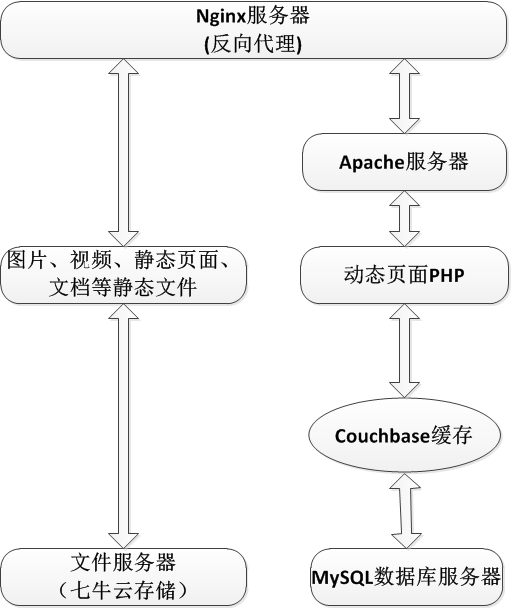
\includegraphics[height=6cm]{./img/web_frame2.png}
    \caption{平台基本框架}
    \label{fig:visual}
  \end{figure}
\end{frame}

\begin{frame}
\frametitle{二、\cite{crab1}推荐系统研究与开发}
  \begin{block}{本课题使用的推荐算法和框架}
    \begin{itemize}
      \item 本课题主要使用协同过滤推荐算法中的基于用户的协同过滤算法
      \item \cite{crab2}本课题使用的框架是基于Python的Crab推荐系统引擎
    \end{itemize}
  \end{block}
  \begin{block}{协同过滤推荐算法(Collaborative Filtering Recommendation)}
    \begin{itemize}
      \item 基于用户的协同过滤(User-Based CF)\\
      找到和目标用户兴趣相似的用户集合,然后给目标用户推荐这个集合的用户喜欢的物品
      \item 基于物品的协同过滤(Item-Based CF)\\
      给目标用户推荐与他喜欢的物品相似度较高高的物品\\
    \end{itemize}
  \end{block}
\end{frame}

\begin{frame}
\frametitle{基于用户的协同过滤算法的主要公式和步骤}
  \begin{itemize}
    \item \cite{crab3} 基于用户的协同过滤的关键在于计算用户与用户之间的兴趣相似度,主要使用余弦相似度来计算:\\
    \begin{displaymath}
    \omega_{\mu\nu} = \frac{|N(\mu) \cap N(\nu)|}{\sqrt{|N(\mu) \parallel N(\nu)|}}
    \end{displaymath}
    $\omega_{\mu\nu}$代表用户 $\mu$ 与 $ \nu $ 之间的兴趣相似度,$ {N(\mu)} $ 表示用户 $ \mu $ 曾经喜欢过的物品集合, $ {N(\nu)} $ 表示用户 $ \nu $ 曾经喜欢过的物品集合
    \item 根据上述描述,可以有如下算法步骤
      \begin{enumerate}
        \item 建立物品-用户的倒排表(Inverted Index)
        \item 计算用户与用户之间的共享矩阵 $C[\mu][\nu]$,表示用户$\mu$与$\nu$喜欢相同物品的个数
        \item 计算用户与用户之间的相似度矩阵 $\omega[\mu][\nu]$,根据上述相似度计算公式计算
        \item 用上面的相似度矩阵来给用户推荐和他兴趣相似的用户喜欢的物品
      \end{enumerate}
  \end{itemize}
\end{frame}

\begin{frame}
\frametitle{二、推荐系统研究与开发}
  \begin{block}{Crab推荐系统引擎}
    \begin{itemize}
      \item Crab是基于Python开发的开源推荐软件,其中实现的方法有item和user的协同过滤
      \item 基于scikit-learn库(Python下的一个机器学习库),建立在NumPy,SciPy和matplotlib模块之上,为用户提供各种机器学习算法接口
    \end{itemize}
  \end{block}
  \begin{figure}
    \centering
      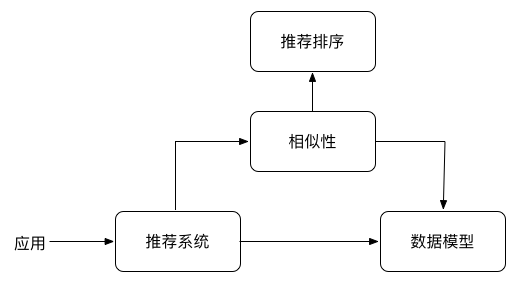
\includegraphics[height=3cm]{./img/crab.png}
    \caption{crab框架}
    \label{fig:visual}
  \end{figure}
\end{frame}

\begin{frame}
\frametitle{三、持续集成方案研究}
  \begin{block}{本课题搭建持续集成的目的和研究}
    \begin{itemize}
      \item 在使用持续集成方案之前,系统的部署流程是直接将代码通过GitLab的钩子(hook)将代码同步到服务器端的WEB目录下,没有进行自动化的构建、测试和部署。
    \end{itemize} 
  \end{block}
  \begin{figure}
    \centering
      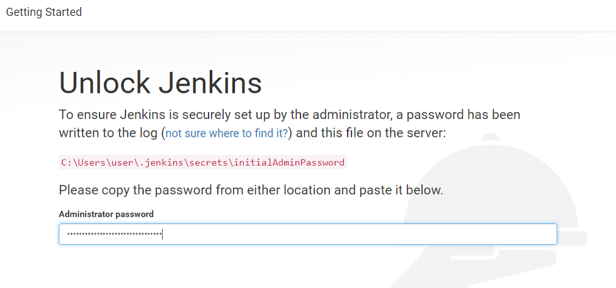
\includegraphics[height=3cm]{./img/jenkins1.png}
    \caption{原部署流程}
    \label{fig:visual}
  \end{figure}
\end{frame}

\begin{frame}
\frametitle{三、持续集成方案研究}
  \begin{block}{本课题搭建持续集成的目的和研究}
    \begin{itemize}
      \item 使用持续集成方案之后,通过GitLab的钩子(hook)触发系统的持续集成工具,对代码进行合并、构建、测试和部署,出现重大问题时可以回滚。
    \end{itemize}
  \end{block}
  \begin{figure}
    \centering
      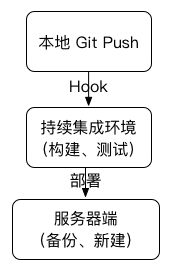
\includegraphics[height=3cm]{./img/jenkins2.png}
    \caption{现部署流程}
    \label{fig:visual}
  \end{figure}
\end{frame}

\begin{frame}
\frametitle{三、持续集成方案研究}
  \begin{block}{关于持续集成}
    持续集成是一种软件开发实践,通过频繁地(一天多次)将代码集成到主干。每次集成都通过自动化的构建(包括编译,发布,自动化测试)来验证,从而尽早地发现集成错误\cite{jenkins1}。
  \end{block}
  \begin{block}{集成环境的搭建和配置}
    \begin{itemize}
      \item 本地搭建Jenkins持续集成服务器,并且安装针对PHP的构建、测试插件
      \item 开发Hook触发脚本和持续部署脚本,实现服务器端的的代码更新和文件备份 
    \end{itemize} 
  \end{block}
\end{frame}

\begin{frame}
\frametitle{四、系统缓存和优化方案研究}
  \begin{itemize}
    \item 系统之前版本和现在版本使用的缓存机制对比
  \end{itemize} 
  \begin{columns}
    \begin{column}{0.50\textwidth}
      \begin{figure}
        \centering
          
\includegraphics[height=4cm]{./img/couchbase1.png}
        \caption{之前数据操作模型}
        \label{fig:visual}
      \end{figure}
    \end{column}
    \begin{column}{0.50\textwidth}
      \begin{figure}
        \centering
          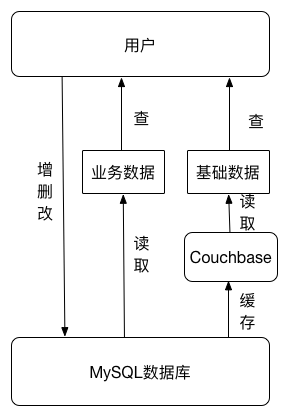
\includegraphics[height=4cm]{./img/couchbase2.png}
        \caption{当前数据操作模型}
        \label{fig:visual}
      \end{figure}
    \end{column}
  \end{columns}
\end{frame}

\begin{frame}
\frametitle{四、系统缓存和优化方案研究}
  \begin{block}{Couchbase缓存\cite{couchbase1} }
    \begin{itemize}
      \item Couchbase是一个高性能以及可用性强的NoSQL数据库引擎
      \item 使用Couchbase将系统的业务数据在系统启动时加载到缓存中,降低系统的丢包率并加快数据读取速度 
    \end{itemize} 
  \end{block}
  \begin{block}{ElasticSearch搜索引擎\cite{elasticsearch1} }
    \begin{itemize}
      \item Elasticsearch是一个基于Apache Lucene(TM)的开源搜索引擎
      \item 实时分析搜索引擎,每个字段都被索引并可被搜索,能够达到搜索实时、稳定、可靠和快速,支持通过HTTP请求,使用JSON进行数据索引\cite{elasticsearch2}
    \end{itemize} 
  \end{block}
\end{frame}

\begin{frame}
\frametitle{四、系统缓存和优化方案研究}
  \begin{block}{七牛云存储}
    \begin{itemize}
      \item 将平台的图片和视频等媒体数据上传到七牛云存储
      \item 通过七牛的CND加速加快系统图片和视频的加载速度
    \end{itemize} 
  \end{block}
  \begin{block}{WEB缓存的意义和作用}
    \begin{itemize}
      \item 减少网络带宽消耗
      \item 降低服务器压力
      \item 减少网络延迟,加快页面打开速度
    \end{itemize} 
  \end{block}
\end{frame}
%% ++++++++++++++++++++++++++++++++++++++++++++++++++++++
%%      进展情况
%% ++++++++++++++++++++++++++++++++++++++++++++++++++++++
\begin{frame}
\frametitle{后续工作安排}
  \begin{block}{已完成 }
	\begin{itemize}
		\item 平台功能开发
		\item Jenkins自动化测试、部署工具的配置和部署脚本开发
        		\item Couchbase缓存机制的开发
		\item ElasticSearch分布式全文搜索引擎的部署和测试
	\end{itemize}
  \end{block}
  \begin{block}{进行中}
	\begin{itemize}
    \item 缓存和搜索接口的开发
    \item 推荐系统的开发
	\end{itemize}
  \end{block}
\end{frame}

%% ++++++++++++++++++++++++++++++++++++++++++++++++++++++
%%      Last Page
%% ++++++++++++++++++++++++++++++++++++++++++++++++++++++
% \begin{frame}
% \frametitle{大学生创业平台的开发与系统优化策略研究}
%   谢谢各位老师的聆听!
% \end{frame}

%% ++++++++++++++++++++++++++++++++++++++++++++++++++++++
%%      Reference Page
%% ++++++++++++++++++++++++++++++++++++++++++++++++++++++
\begin{frame}[allowframebreaks]{References}
  \scriptsize
  \bibliographystyle{plain}
  \bibliography{myRefs}
\end{frame}

\end{document}
%% ======================================================
